% ****** Start of file apssamp.tex ******
%
%   This file is part of the APS files in the REVTeX 4.1 distribution.
%   Version 4.1r of REVTeX, August 2010
%
%   Copyright (c) 2009, 2010 The American Physical Society.
%
%   See the REVTeX 4 README file for restrictions and more information.
%
% TeX'ing this file requires that you have AMS-LaTeX 2.0 installed
% as well as the rest of the prerequisites for REVTeX 4.1
%
% See the REVTeX 4 README file
% It also requires running BibTeX. The commands are as follows:
%
%  1)  latex apssamp.tex
%  2)  bibtex apssamp
%  3)  latex apssamp.tex
%  4)  latex apssamp.tex
%
\documentclass[%
 reprint,
%superscriptaddress,
%groupedaddress,
%unsortedaddress,
%runinaddress,
%frontmatterverbose,
%preprint,
%showpacs,preprintnumbers,
%nofootinbib,
%nobibnotes,
%bibnotes,
 amsmath,amssymb,
 aps,
%pra,
%prb,
%rmp,
%prstab,
%prstper,
%floatfix,
]{revtex4-1}

\usepackage{float}
\usepackage{graphicx}% Include figure files
\usepackage{dcolumn}% Align table columns on decimal point
\usepackage{bm}% bold math
\usepackage{hyperref}% add hypertext capabilities
%\usepackage[mathlines]{lineno}% Enable numbering of text and display math
%\linenumbers\relax % Commence numbering lines
% \usepackage[toc,page]{appendix}
% \addbibresource{sample.bib}


%\usepackage[showframe,%Uncomment any one of the following lines to test
%%scale=0.7, marginratio={1:1, 2:3}, ignoreall,% default settings
%%text={7in,10in},centering,
%%margin=1.5in,
%%total={6.5in,8.75in}, top=1.2in, left=0.9in, includefoot,
%%height=10in,a5paper,hmargin={3cm,0.8in},
%]{geometry}

\begin{document}

%\preprint{APS/123-QED}

\title{LASSO or $L_1$ regularization in linear models - Appedix}% Force line breaks with \\
% \thanks{Project in Advanced Methods in Applied Statistics}%

\author{Magnus Berg Sletfjerding}
 % \altaffiliation[Also at ]{Physics Department, XYZ University.}%Lines break automatically or can be forced with \\

\affiliation{%
 Copenhagen University
}%

\date{\today}% It is always \today, today,
             %  but any date may be explicitly specified


\maketitle

\begin{figure}[H]
 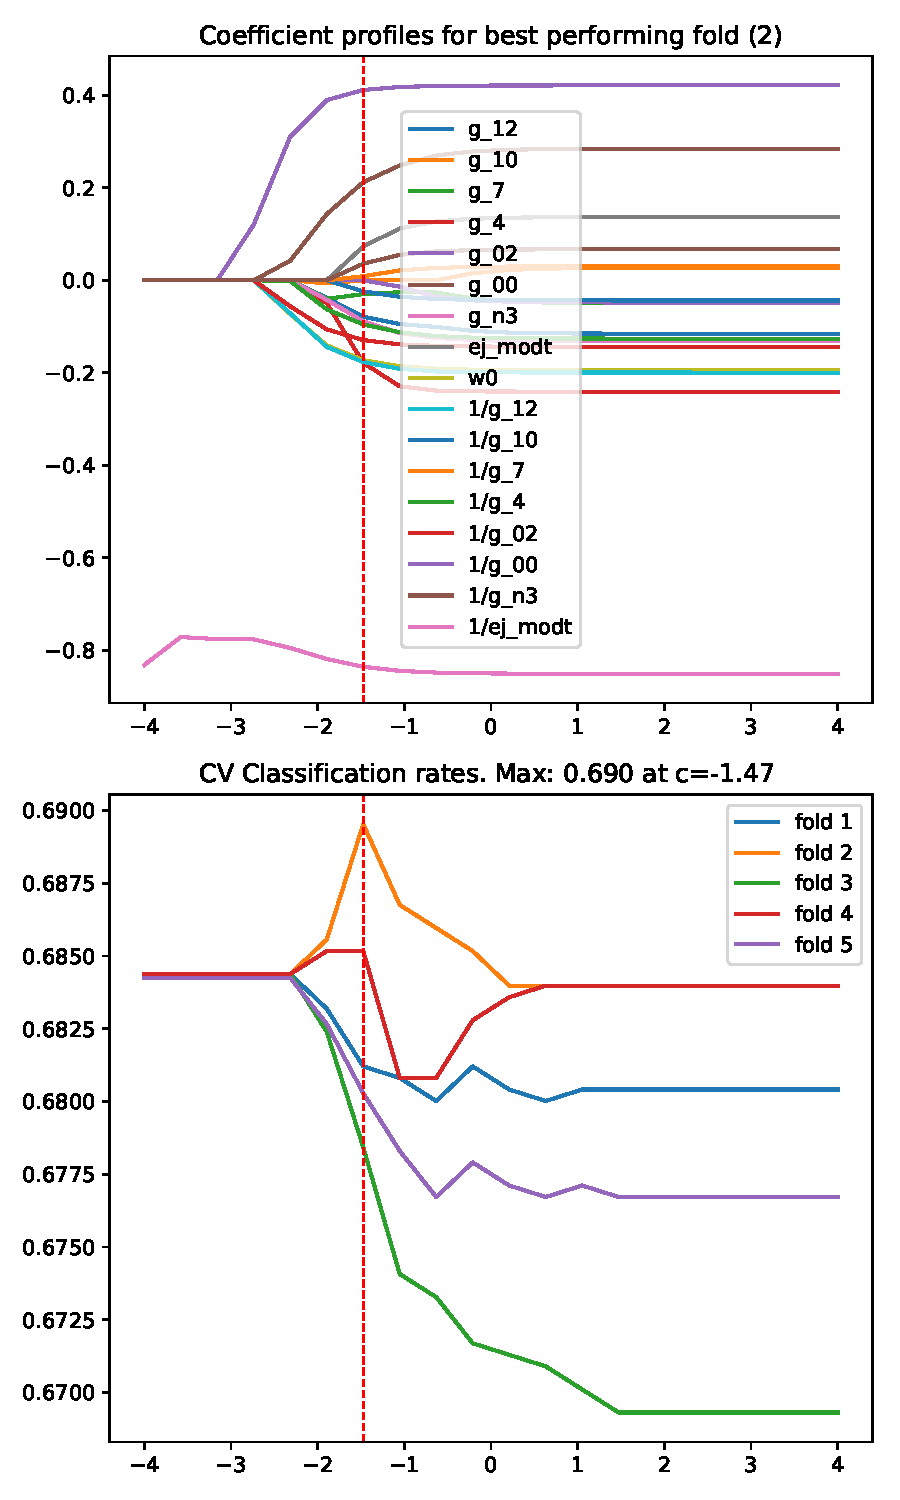
\includegraphics[width=0.9\linewidth]{../figs/LogRegCV_KU_div}
 \caption{L1 Regularized Logistic Regression on KU grade data, with reciprocal features engineered to see if it gave a better accuracy.
 \textbf{Top}: Coefficient paths, for the best performing cross validation fold.
 I used 5 random folds in total.
 \textbf{Bottom}: Classification rates for the 5 folds.
 }
\end{figure}

\begin{figure}[H]
 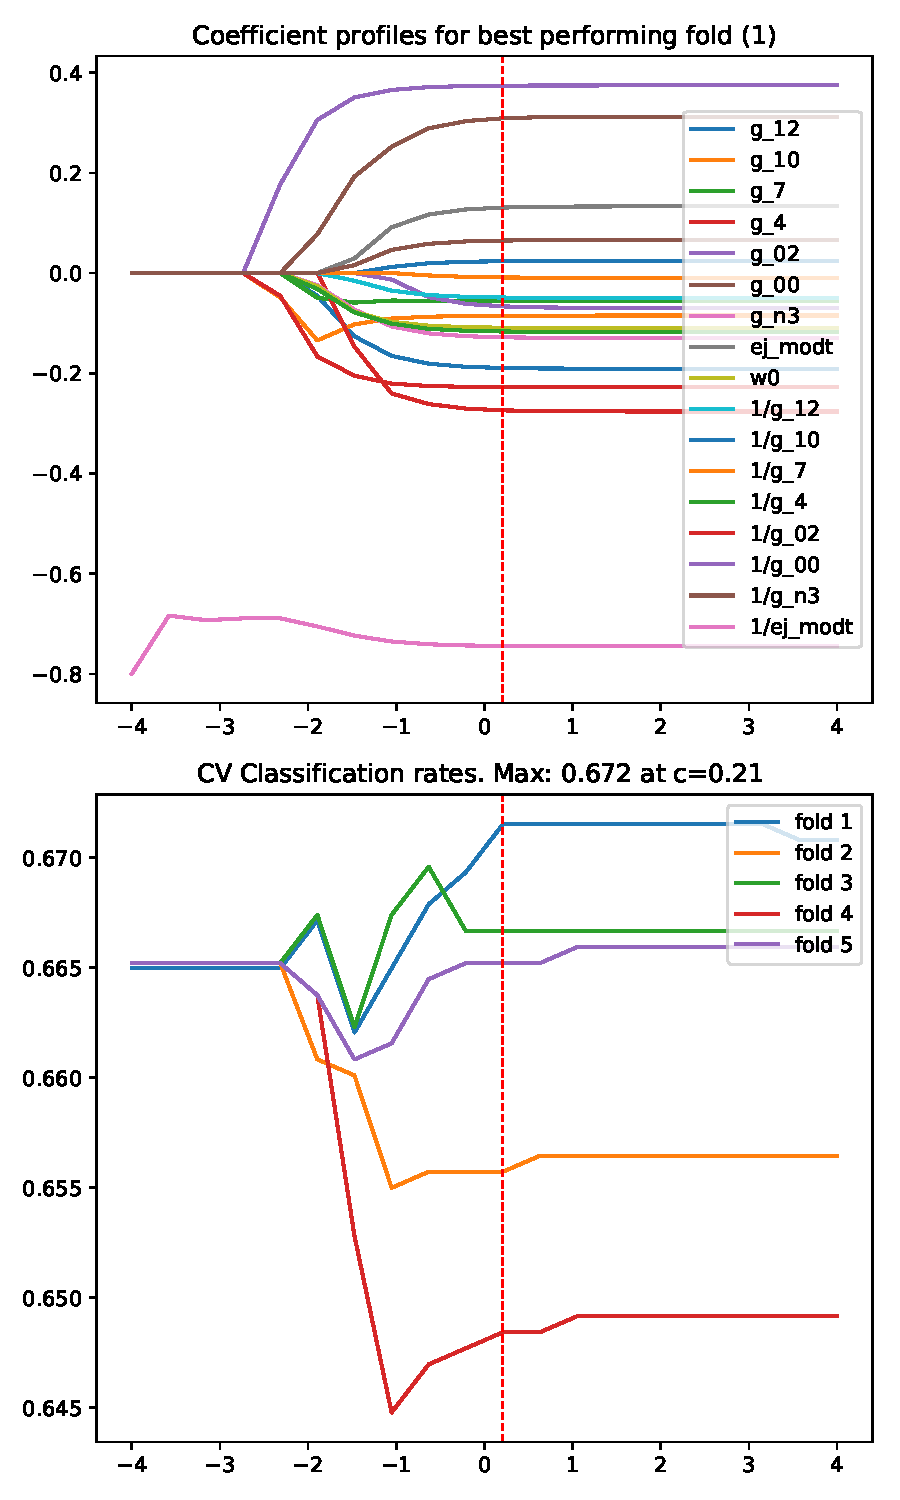
\includegraphics[width=0.9\linewidth]{../figs/LogRegCV_KU_div_participants}
 \caption{L1 Regularized Logistic Regression on KU grade data, with reciprocal features engineered and courses with less than 30 particpants removed.
 \textbf{Top}: Coefficient paths, for the best performing cross validation fold.
 I used 5 random folds in total.
 \textbf{Bottom}: Classification rates for the 5 folds. A slightly better classification rate was found, but not deemed to be significantly above the classification rate found in the main part of the report.
 }
\end{figure}




\end{document}
